\section{Introduction}
\label{sec:intro}
% edited by Steven C. 23-Apr-2019

Observational sciences such as astronomy have long relied on computational resources to extract scientific discoveries from measurements. 
Since cause and effect cannot be studied directly with controlled experiments, expert analysis of observational data is the only way that processes which cannot be interacted with can be understood. 
This is true in the field of heliophysics whose goal is to understand the Sun and its interactions with Earth and the solar system. 
This field combines a number of sub-disciplines such as solar physics, ionospheric and magnetospheric physics. 
In order to advance our understanding of the fundamental processes underpinning this complex system, interdisciplinary research across these scientific disciplines is required. 
At the time of writing, the NASA-operated Heliophysics Systems Observatory consists of 18 operating missions with 24 spacecraft and 5 missions current under development.  
Software packages to analyze these datasets have generally been developed independently by projects teams. 
The result of this approach is a diverse and therefore difficult data and software environment to navigate. 
A common platform that addresses simple tasks, provides a standard interface to data products, and encourages re-use of common functions can go a long way toward solving this problem. 
SunPy is a project which aims to provide this solution for the field of solar physics. 
\todo{the problem needs to be properly defined - i.e. difficult for users, no common platform, non-consistent, reproducibility etc.}

The mission statement of the \sunpyproj is to facilitate and promote the use and development of a community-led, free and open-source\footnote{https://opensource.org/osd} data-analysis software based on the scientific \python\footnote{\url{https://www.python.org/}} environment. 
To achieve that goal, the project develops and maintains a core package (\sunpypkg) and supports an ecosystem of affiliated packages (see \ref{sec:affil_packages}) that provide additional functionality. 
The project was formally founded in March of 2014 though development of the core package began three years earlier. 
\citet{Community:2015cy} describes version 0.5 which was released in June 2014.

The \sunpyproj selected \python to leverage the rich ecosystem of packages available for general data analysis. 
These include packages such as \package{Numpy} which provides efficient multi-dimensional numerical array manipulation \citep{numpy} ; \package{scipy} which provides fundamental scientific functions such as for numerical integration and optimization\citep{scipy}; \package{Matplotlib} provides publication-ready 2D plotting \citep{matplotlib}, and finally \package{Pandas} provides data structures and analysis support with support for time series \citep{pandas}.
These packages form the foundation of the scientific \python ecosystem. 
Together they represent $>$500,000 lines of code\footnote{As measured by cloc (\url{github.com/AlDanial/cloc})}. 
Significant additional packages have been developed which depend on these foundational packages. 
Of particular relevance to \sunpypkg is the \astropypkg package which provides core functionality for astronomy \citep{astropy2018}. 

%The project began as a community-led effort to organize and standardize existing functionality and also to provide a \todo{Would "open source" be better than "free" because SSW is "free" but it's not "open source" - SJM} free and modern alternative to the existing SolarSoft (SSW, \citet{Freeland:1998we}) software package. While SSW is open source and freely available, it is primarily composed of source code for the Interactive Data Language (IDL), a proprietary data-analysis environment currently owned by Harris Geospatial Solutions. In addition, the development of SSW is not open to the community and is not version controlled.



%NumPy 102906 LOC
%SciPy 139009 LOC
%matplotlib 98720 LOC
%pandas 212338 LOC
%astropy 151825 LOC

%The SunPy Project aims to develop and provide high-quality, maintainable and tested code paired with extensive documentation that follow current best practices in software development. 

%The core library sets a standard and example for other codes to follow.

%A description of the current affiliated packages can be found in Section~\ref{sec:affil_packages}.

\section{Project Organization \& Enhancement Proposals - Steven Christe}
% edited by Steven C. 23-Apr-2019

The organization of the \sunpyproj is modeled on the structure of a board-only not-for-profit corporate entity. 
It consists of an up-to 10 member self-selected board. 
An executive director, elected by the board, is the lead developer whose responsibilities include leading the developer community, providing user support, developing and maintaining the core package, as well as supporting the development of affiliated packages. 
The lead developer is supported by a deputy as well as other volunteers from the developer community. 
Board members serve two year terms while the lead developer serves one year terms. 

The \sunpyproj is formally defined through \sunpy Enhancement Proposals (SEPs) which are modeled after the Python Enhancement Proposal process\footnote{\url{https://www.python.org/dev/peps/}}. 
The first two SEPs (SEP-0001 and SEP-0002) define themselves as well as the \sunpy organization. 
They are version controlled and publicly available\footnote{\url{https://github.com/sunpy/sunpy-SEP}}. 
SEPs are both used to define the project as well as requirements on the the \sunpypkg package. 
There are generally three types of SEPs. 
\begin{itemize}
    \item \textbf{Standard}: Introduces and describes a new feature or changes to an existing feature (e.g. API change) and is meant to function as a high-level design document.
    \item \textbf{Process}: describes a new process or a change to an existing process in the management of the project. Examples include procedures, guidelines, changes to the decision-making process or management structure, and changes to the tools or environment.
    \item \textbf{Informational}: Provides information and does not introduce any new features or changes nor describes a new process.
\end{itemize}

As of the time of writing, there are a total of 8 SEPs. 
Some notables SEPs have lead to the adoption of physical units throughout the code base (SEP-0003, see Section~\ref{sec:units}), defined the affiliated package program (SEP-0004, see Section~\ref{sec:affil_package}), standardized the use of coordinate and coordinate transformations (SEP-0005, see Section~\ref{sec:coords}), and led to the adoption of a high precision scientific time format (SEP-0008).

\section{Support \& Sustainability}
% edited by Steven C. 23-Apr-2019

The \sunpyproj relies largely on unpaid, volunteer efforts from early-career scientists which donate their time sometimes as part of their regular work duties.
The \sunpy project has not received any significant direct financial support for its work facilitating and promoting open-source and open development software including developing the \sunpypkg. 

Some development was funded by the Google Summer of Code (GSOC) and the ESA Summer of Code in Space (SOCIS) as well as a small grant from NumFOCUS. 
\todo{sdc - point to a list of all students, isn't this available on sunpy.org?}
\todo{Not sure if its full list but we have this: https://github.com/sunpy/sunpy/wiki/Wall-of-Fame}

Further, these developers receive little to no formal recognition for their work \citep{Muna2016}. 
\todo{sdc - doesn't really flow, we are talking about funding here, not recognition}
This situation is similar to that faced by the \astropy project \citep{PriceWhelan:2018ji}. 
The National Academies of Sciences, Engineering, and Medicine's 2018 report on Open Source Software Policy Options for NASA Earth and Space Sciences \citep{NAP2018} outlines several solutions to alleviate this problem -- namely that the NASA Science Mission Directorate provide funding for new and existing open source software projects, promote scientists who spend time developing and improving open source software projects, and offer prizes for exemplary contributions to the open source software community. 
The \sunpy community supports solutions like these for all relevant funding agencies and furthermore has the ability to accept financial contributions from institutions or individuals through the NumFOCUS organization.

\section{Development Model - NABIL}
% edited by Steven C. 23-Apr-2019

To satisfy the mission statement of the project an open development model was adopted for all development. 
This development model is widely used within the scientific Python community. 
The \sunpy organization and \sunpypkg package are hosted on \github and use Git (\url{https://git-scm.com/}) as its distributed version control software.
The entire codebase is publicly available and anyone can suggest changes through pull requests. 
Furthermore, the codebase is licensed under a permissive 2-clause BSD licence (\url{https://opensource.org/licenses/BSD-2-Clause}), therefore anyone can redistribute, improve, repackage or use it in a closed environment as long as the copyright notice and the license disclaimer about the warranty are maintained. 
In order to maintain a high quality code any contribution much satisfy the following requirements.
\begin{enumerate}
    \item Code and documentation must follow widely used style guides (PEP 8 and numpydoc).
    \item Documentation must be provided with all new features which includes code comments, formal documentation and gallery examples.
    \item Test code must be provided with coverage at or above X\%.
\end{enumerate}
Finally all code must be reviewed and accepted by at least two members of the developer community before they are accepted into the codebase. 

\begin{figure}
\begin{tabular}{ccc}
  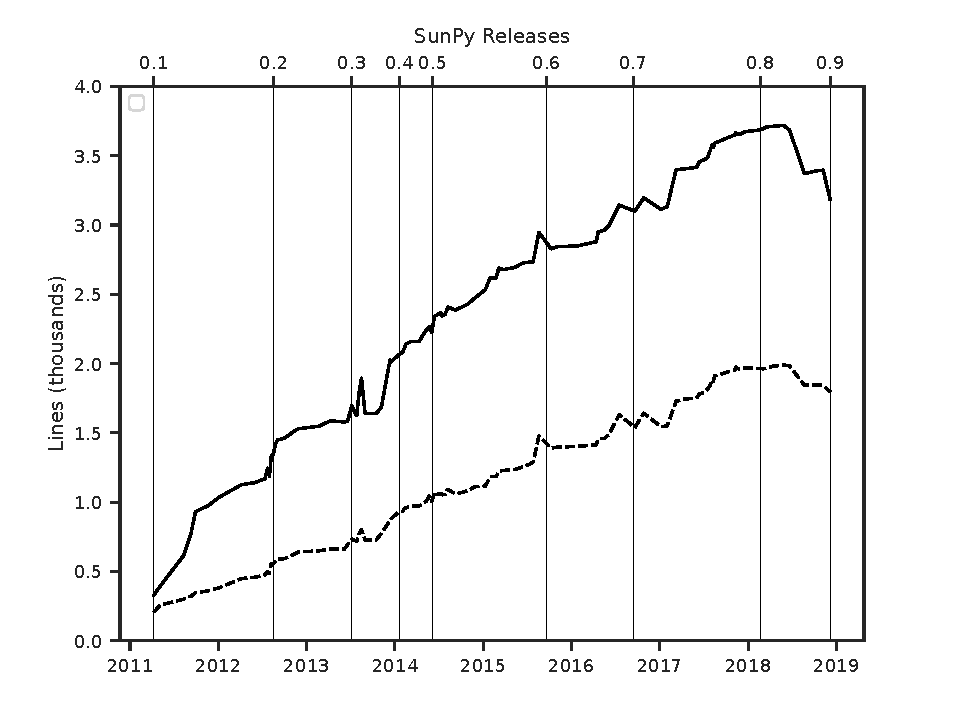
\includegraphics[width=45mm]{figures/sunpy_history.pdf} &
  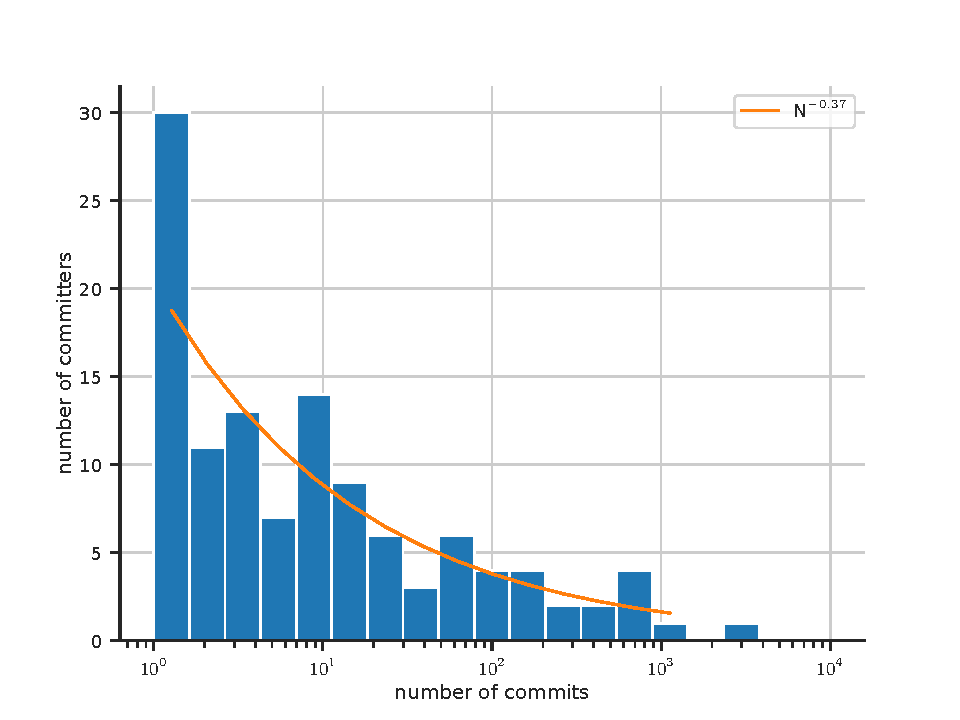
\includegraphics[width=45mm]{figures/busfactor_plot.pdf} &   
  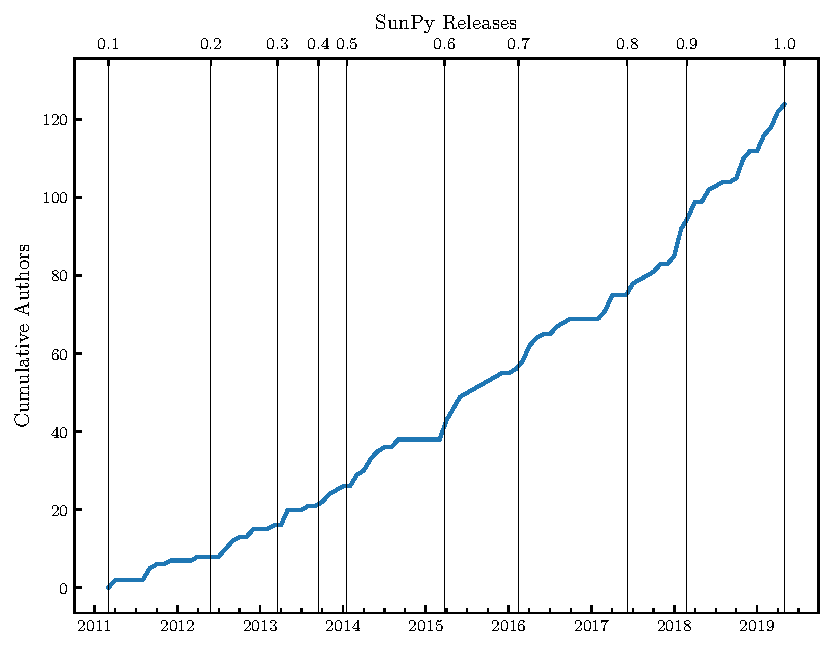
\includegraphics[width=45mm]{figures/cumulative_authors.pdf} \\
(a) & (b) & (c) \\
\end{tabular}
\caption{(a) The }
\label{fig:image2}
\end{figure}

